\documentclass[ALICE,manyauthors]{ALICE_analysis_notes}
%\documentclass[ALICE,manyauthors]{ALICE_scientific_notes}
%
%\newcommand{\jpsi}{\rm J/$\psi$}
%\newcommand{\psip}{$\psi^\prime$}
%\newcommand{\jpsiDY}{\rm J/$\psi$\,/\,DY}
%\newcommand{\dd}{\mathrm{d}}
%\newcommand{\chic}{$\chi_{\rm c}$}
%\newcommand{\ezdc}{$E_{\rm ZDC}$}
%\newcommand{\red}{\textcolor{red}}
%\newcommand{\blue}{\textcolor{blue}}
\newcommand{\slfrac}[2]{\left.#1\right/#2}
\newcommand{\pap}{$\rm p\bar{\rm p}$}
\newcommand{\pal}{$\rm p\bar{\rm \Lambda}$}
\newcommand{\apl}{$\bar{\rm p }\Lambda$}
\newcommand{\ap}{$\bar{\rm p }$}
\newcommand{\p}{$\rm p $}
\newcommand{\aL}{$\bar{\Lambda}$}

\usepackage{rotating}
%
\begin{document}%
%%%%%%%%%%%%% ptdr definitions %%%%%%%%%%%%%%%%%%%%%
%
%%%%%%%%%%%%%%%  Title page %%%%%%%%%%%%%%%%%%%%%%%%
%
\begin{titlepage}
  %
  \PHnumber{ALICE-ANA-2014-xxx} 
  \PHdate{\today}
  %
  %%% Put your own title + short title here:
  \title{Baryon-antibaryon (\pap,~\pal,~\apl) femtoscopic correlations in Pb--Pb collisions at $\sqrt{s_{\mathrm{NN}}}=2{.}76$~TeV}
  \ShortTitle{Baryon-antibaryon femtoscopy}   % appears on right page headers
  %
  \author{Dominik Aromi\'nski$^{1}$, Adam Kisiel$^{1}$, Maciej Szyma\'nski$^{1}$}
  \author{
    1. Warsaw University of Technology\\
  }
  \author{Email: maszyman@cern.ch}
  %
  \ShortAuthor{ALICE Analysis Note 2012}      % appears on left page headers, do not change
  %
  \begin{abstract}
    Here goes your abstract 
  \end{abstract}
\end{titlepage}
%
%% \newpage
\section{Introduction}
\label{sec:overview}
In the analysis, we present the measurements of baryon-antibaryon correlations in Pb--Pb collisions at $\sqrt{s_{\mathrm{NN}}}=2.76$~TeV registered by the ALICE experiment. The method of two-particle correlations (commonly referred to as \emph{femtoscopy})  allows for extracting the space-time characteristics of the emitting source created in heavy-ion collision. Using this technique one can also attempt to extract paramters of strong interaction~\cite{}.

\section{Data analysis}
\label{sec:analysis}
\subsection{Data sample}
\subsubsection{Data selection}
The data used in this note come from Pb--Pb collisions recorded by the ALICE experiment during the 2011 run at the LHC (production LHC11h, pass 2). Analysis Object Data (AOD115) files have been used in studies. About 35 milion events have been analysed. The following runs have been used
% only runs with negative magnetic field polarity - \emph{field$--$},
(they correspond to the uniform acceptance - LHC11h\_AOD145\ (runlist 1 - full TPC Flow) dataset from  CF\_PbPb analysis train):

167915, 168115, 168460, 169035, 169238, 169859, 170228 , 167920, 168310, 168464, 169091, 169411, 169923, 170230, 167985, 168311, 168467, 169094, 169415, 170027, 170268, 167987, 168322, 168511, 169138, 169417, 170081, 170269, 167988, 168325, 168512, 169144, 169835, 170155, 170270, 168069, 168341, 168514, 169145, 169837, 170159, 170306, 168076, 168342, 168777, 169148, 169838, 170163, 170308, 168105, 168361, 168826, 169156, 169846, 170193, 170309, 168107, 168362, 168988, 169160, 169855, 170203, 168108 , 168458, 168992, 169167, 169858, 170204

% Also, the data collected in the 2010 were used for comparison. The following runs have been used (LHC10h\_AOD086 dataset from  CF\_PbPb analysis train):

% 139510, 139507, 139505, 139503, 139465, 139438, 139437, 139360, 139329, 139328, 139314, 139310, 139309, 139173, 139107, 139105, 139038, 139037, 139036, 139029, 139028, 138872, 138871, 138870, 138837, 138732, 138730, 138666, 138662, 138653, 138652, 138638, 138624, 138621, 138583, 138582, 138579, 138578, 138534, 138469, 138442, 138439, 138438, 138396, 138364, 138275, 138225, 138201, 138197, 138192, 138190, 137848, 137844, 137752, 137751, 137724, 137722, 137718, 137704, 137693, 137692, 137691, 137686, 137685, 137639, 137638, 137608, 137595, 137549, 137544, 137541, 137539, 137443, 137441, 137440, 137439, 137434, 137432, 137431, 137430, 137366, 137243, 137236, 137235, 137232, 137231, 137230, 137162, 137161, 137135

The analysis was done as a part of the ``Lego Trains''.
% 169591, 169588, 169586, 169557, 169550, 169512, 169504, 169498, 169475, 169419, 169418, 169417, 169415, 169411, 169238, 169167, 169160, 169156, 169148, 169145, 169144, 169138, 169099, 169094, 169091, 169044, 169035, 168992, 168988, 168826, 168777, 168514, 168512, 168511, 168464, 168460, 168458, 168362, 168361, 168342, 168341, 168325, 168322, 168311, 168310, 168115, 168108, 168107, 168105, 168076, 168069, 167988, 167987, 167985, 167920, 167915

\subsubsection{Monte Carlo}
We used the HIJING production LHC11a10a\_bis (AOD120) and AMPT production LHC12a17a (AOD110).
\subsection{Analysis software}
The analysis was performed using the \verb|AliFemto| package being a part of \verb|AliROOT|.%  framework (v5-03-34-AN):

% \verb|http://alisoft.cern.ch/viewvc/tags/v5-03-34-AN/PWGCF/FEMTOSCOPY/|
%.

\subsection{Event selection}


\subsection{Particle identification}
\subsubsection{(Anti-)protons identification}
\subsubsection{(Anti-)lambdas identification}


\subsection{Track selection}


\subsection{Pair selection}

\subsection{Correlation functions}


\section{Results}


\subsection{Correlation functions}


\subsubsection{Momentum resolution correction}


\subsection{Fitting}
%% \section{Summary}
%% \label{sec:summary}
% In summary, correlations of all combinations of pairs of protons and antiprotons have been measured in Pb--Pb collisions at $\sqrt{s_{\mathrm{NN}}}=2.76$~TeV in the ALICE experiment. The femtoscopic parameters for the radius of the proton source are extracted from one-dimensional pp, $\bar{\mathrm{p}}\bar{\mathrm{p}}$ and p$\bar{\mathrm{p}}$ correlation functions. The fit includes final-state interactions and quantum statistics for identical pairs of (anti)protons. The fit takes into account residual correlations coming from p$\Lambda$ system. Two-proton correlations show an increase of the radius with increasing multiplicity and slight decrease of the radius with increasing  pair transverse momentum. %Also, transverse mass scaling is observed between $\pi\pi$, K$^{\mathrm{ch}}$K$^{\mathrm{ch}}$, \Kzs\Kzs~and two-proton invariant radii.

\begin{thebibliography}{99}
\bibitem{Mercado} The ALICE Collaboration: \emph{Two-pion Bose-Einstein correlations in central PbPb collisions at $\sqrt{s_{\mathrm{NN}}} = 2.76$~TeV}; Phys.Lett.B696:328-337,2011
\bibitem{HZ} Gos,~H.~P. for the STAR collaboration : \emph{Proton - proton, anti-proton - anti-proton, proton - anti-proton correlations in Au+Au collisions measured by STAR at RHIC}; Eur.Phys.J. C49 (2007) 75-80
\bibitem{therminator} Kisiel,~A., Taluc,~T., Broniowski~W., Florkowski,~W.; \emph{THERMINATOR: THERMal heavy-IoN generATOR}; Comput.Phys.Commun. 174 (2006) 669-687
\bibitem{corrfit} Kisiel,~A.: \emph{CorrFit - a program to fit arbitrary correlation functions}; Nukleonika 49;Suppl 2:s81-s83 (2004)
  % \bibitem{llCorinne} Lednicky,~R., Lyuboshitz,~V.~L.: \emph{Final state interaction effect on correlations in narrow particles pairs}; In *Nantes 1990, Proceedings, Particle correlations and interferometry in nuclear collisions* 42-54
\bibitem{LednickyDirac} Lednicky,~R.: \emph{Finite-size effects on two-particle production in continuous and discrete spectrum}; Phys.Part.Nucl. 40 (2009) 307-352
\bibitem{ak_savannah_bug} The LHC Computing Grid software development portal Savannah: \url{https://savannah.cern.ch/bugs/?func=detailitem&item_id=75267}
\bibitem{CKB} Christian Klein-Boesing, private communication
\bibitem{lmalinin} Malinina,~L.: \url{https://indico.cern.ch/getFile.py/access?contribId=22&sessionId=6&resId=0&materialId=slides&confId=147108}
\bibitem{phistar}Gramling,~J.L. \url{http://indico.cern.ch/getFile.py/access?contribId=42&sessionId=16&resId=0&materialId=slides&confId=146554}%\emph{Two-track resolution effects for HBT analyses in ALICE}; ALICE-INT-2011-003

\end{thebibliography}
               %%%%%%%%%%% put the body of the article here

\section{Introduction}
\label{sec:overview}
In the analysis, we present the measurements of baryon-antibaryon correlations in Pb--Pb collisions at $\sqrt{s_{\mathrm{NN}}}=2.76$~TeV registered by the ALICE experiment. The method of two-particle correlations (commonly referred to as \emph{femtoscopy})  allows for extracting the space-time characteristics of the emitting source created in heavy-ion collision. Using this technique one can also attempt to extract paramters of strong interaction~\cite{Kisiel:2014mma}.

\section{Data analysis}
\label{sec:analysis}

\subsection{Data sample}

\subsubsection{Data selection}

\subsubsection{Monte Carlo}

\subsection{Event selection}

\subsection{Particle identification}
QA plots needed

\subsubsection{(Anti-)protons identification}

\subsubsection{(Anti-)lambdas identification}

\subsection{Track selection}

\subsection{Pair selection}

\subsection{Proton and lambda fraction with respect to their origin}
In order to estimate fraction of protons and lambdas coming from certain parent particles was calculated using Monte Carlo Hijing LHC12a17afix. Fractions were checked before reconstruction (pure Monte Carlo) as well as after Geant simulation. Kinematic cuts were applied with the same values as in collision data. It was noticed that before reconstruction, there is a significant contribution of protons at low $p_{T}$  with PDG of mothers corresponding to $\pi$, $K^0_L$, $K^0_S$, $K^+$, $D^+_S$, $J/\psi$, $B^0$, $B^+$, $B^0_S$ which presumably come from interactions with material. Results were also cross checked with Therminator2 simulation without reconstruction stage. Results are show in Fig.~\ref{}

 \begin{figure}[h!]
   \centering
   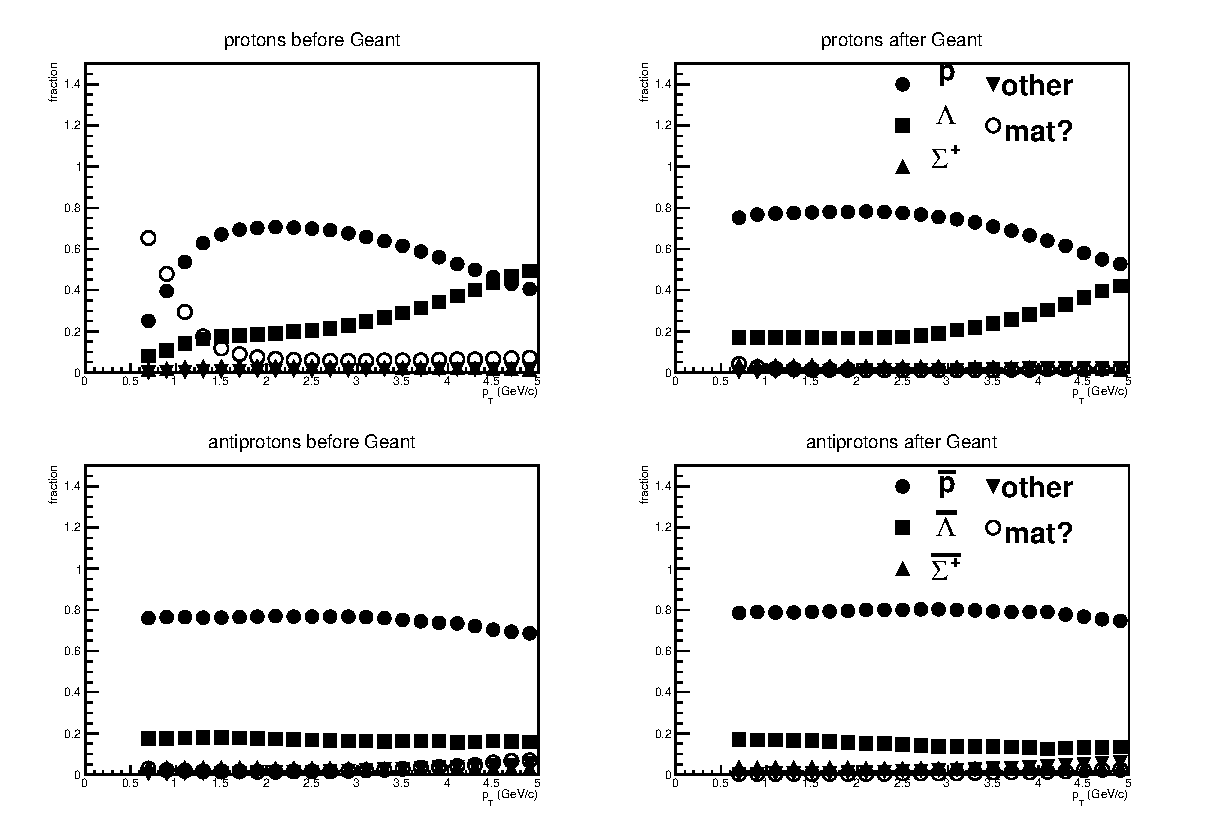
\includegraphics[width=0.99\textwidth]{pics/protonOrigin}
   \caption{Hijing p fraction}
   \label{fig:ProtonFraction}
 \end{figure}

 \begin{figure}[h!]
   \centering
   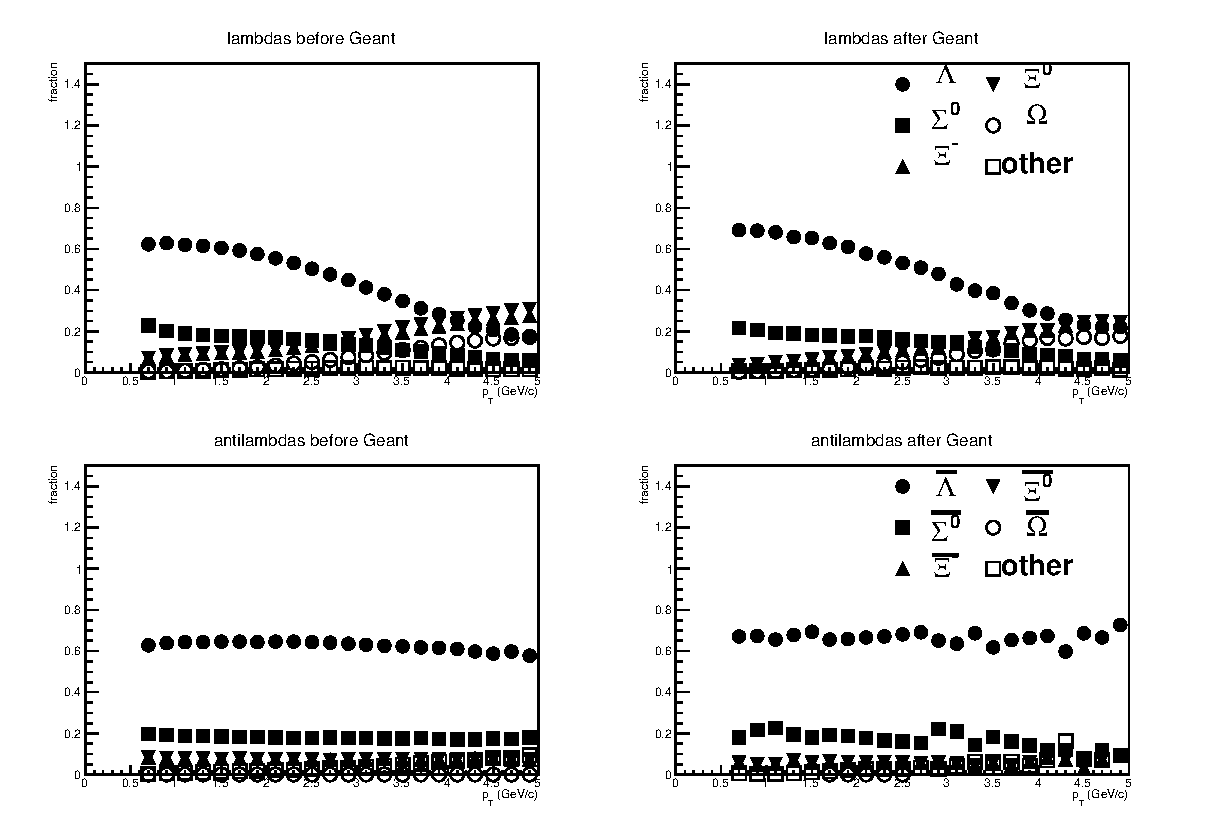
\includegraphics[width=0.99\textwidth]{pics/lambdaOrigin}
   \caption{Hijing $\Lambda$ fraction}
   \label{fig:LambdaFraction}
 \end{figure}

 \begin{figure}[h!]
   \centering
   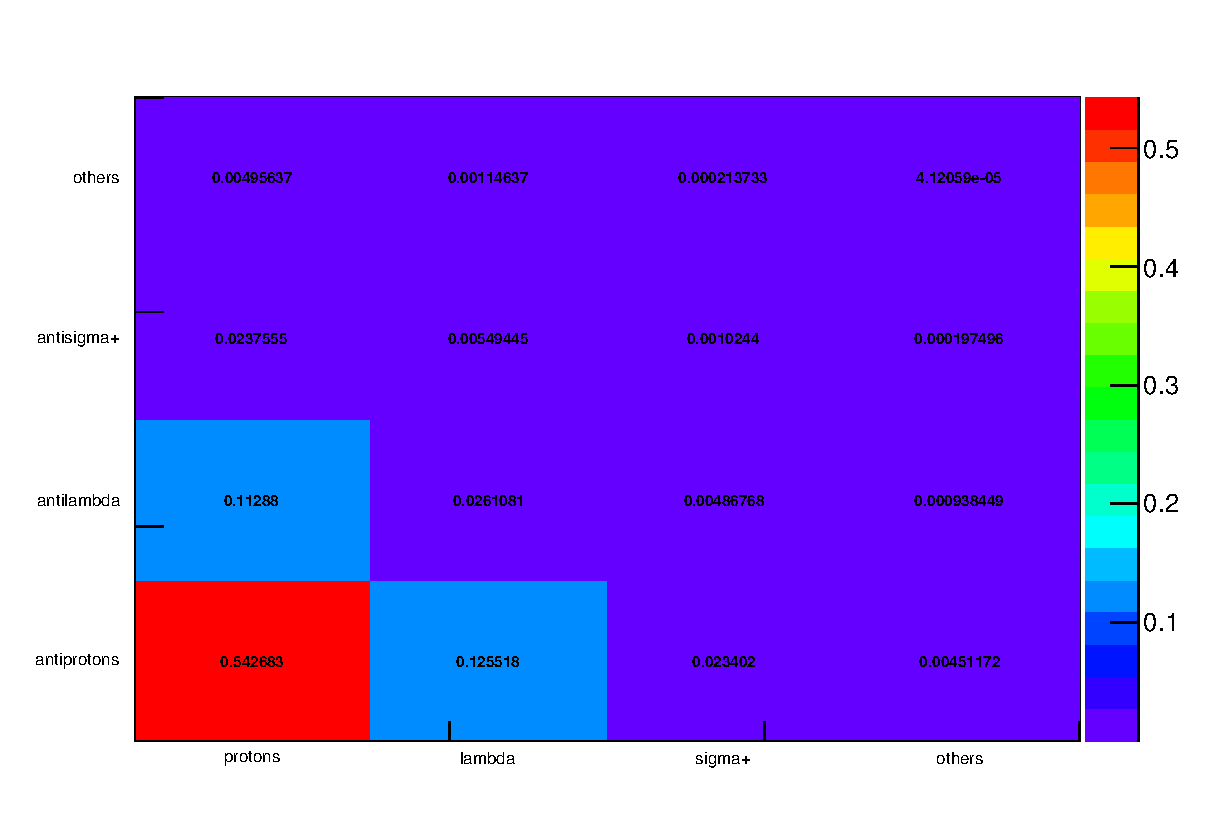
\includegraphics[width=0.99\textwidth]{pics/papFraction}
   \caption{Hijing+Geant ~\pap~Fraction $p_T$ integrated, taking into account 0.95 \p~and \ap~PID purity}
   \label{fig:papFraction}
 \end{figure}

 \begin{figure}[h!]
   \centering
   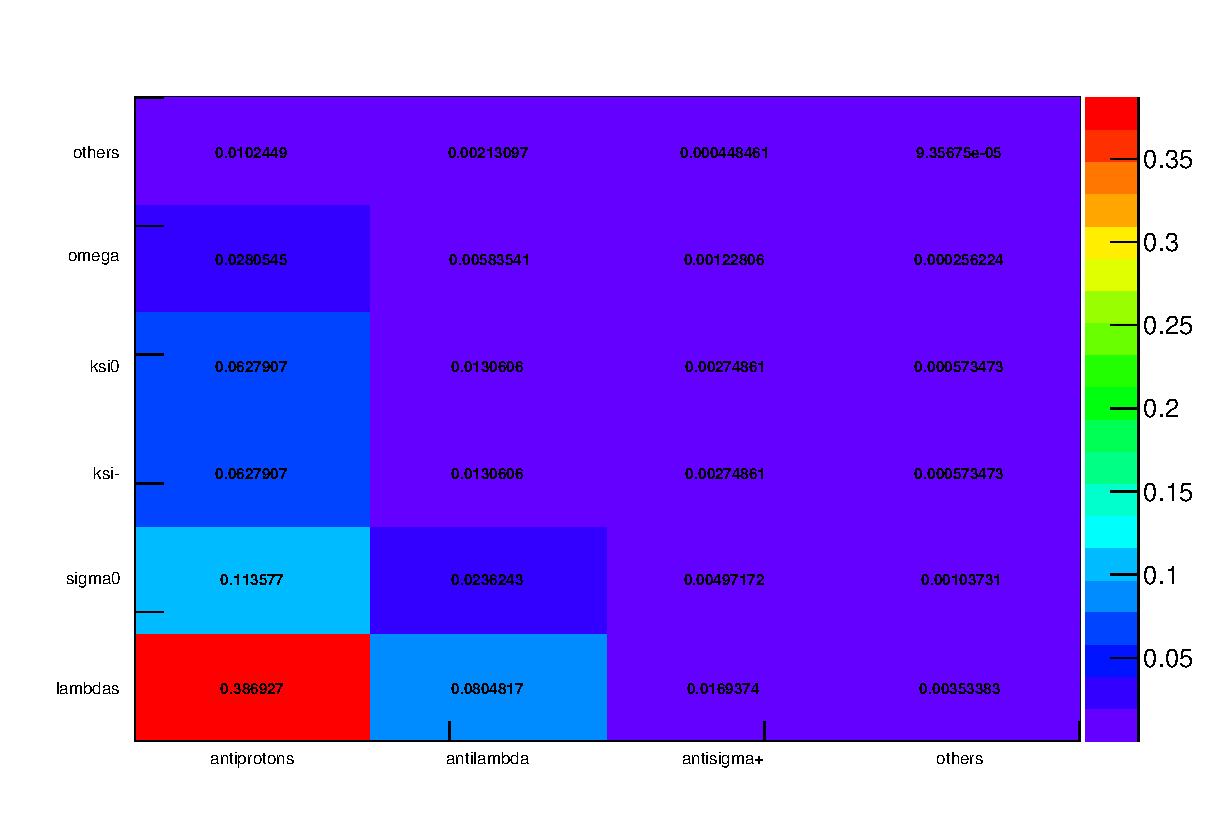
\includegraphics[width=0.99\textwidth]{pics/aplFraction}
   \caption{Hijing+Geant \apl~Fraction $p_T$ integrated, taking into account 0.95 \ap~PID purity and 0.9 $\Lambda$ purity}
   \label{fig:aplFraction}
 \end{figure}

 \begin{figure}[h!]
   \centering
   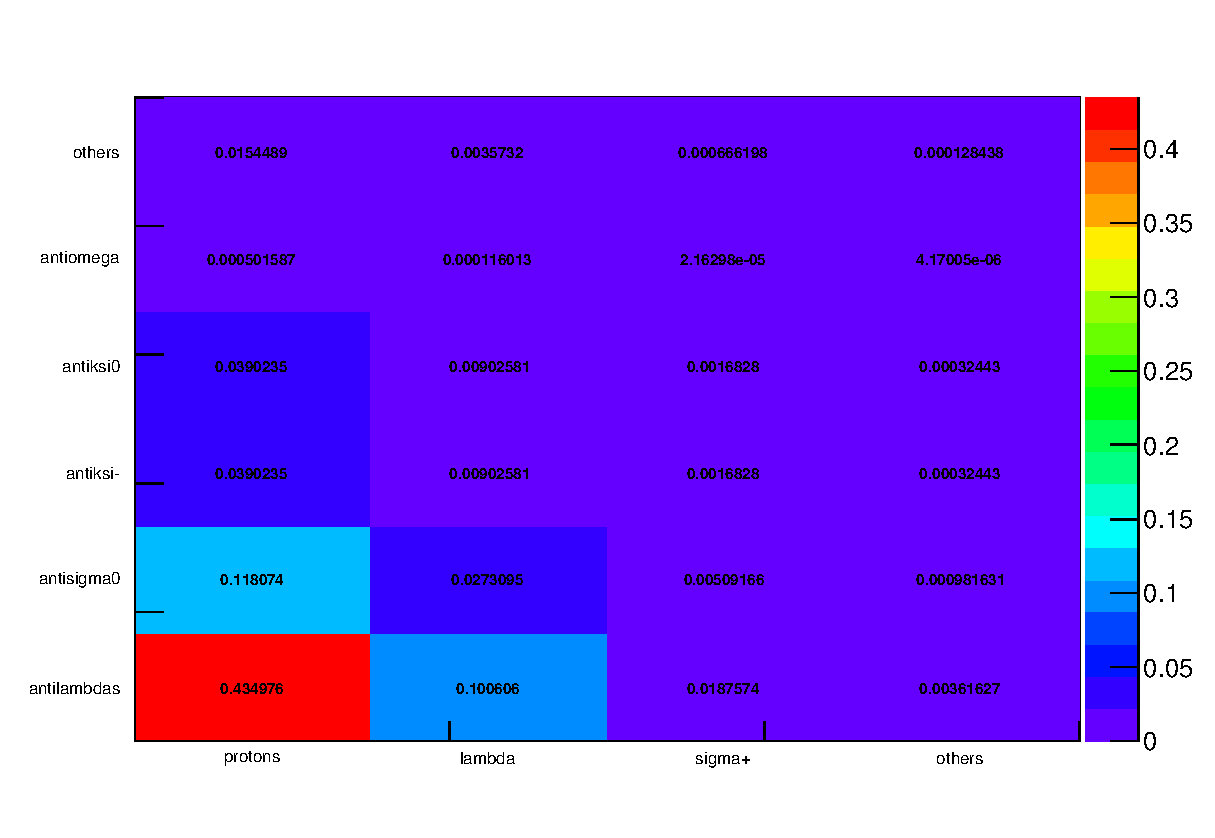
\includegraphics[width=0.99\textwidth]{pics/palFraction}
   \caption{Hijing+Geant \pal~Fraction $p_T$ integrated, 0.95 \p~PID purity and 0.9 \aL~purity}
   \label{fig:palFraction}
 \end{figure}

 \begin{figure}[h!]
   \centering
   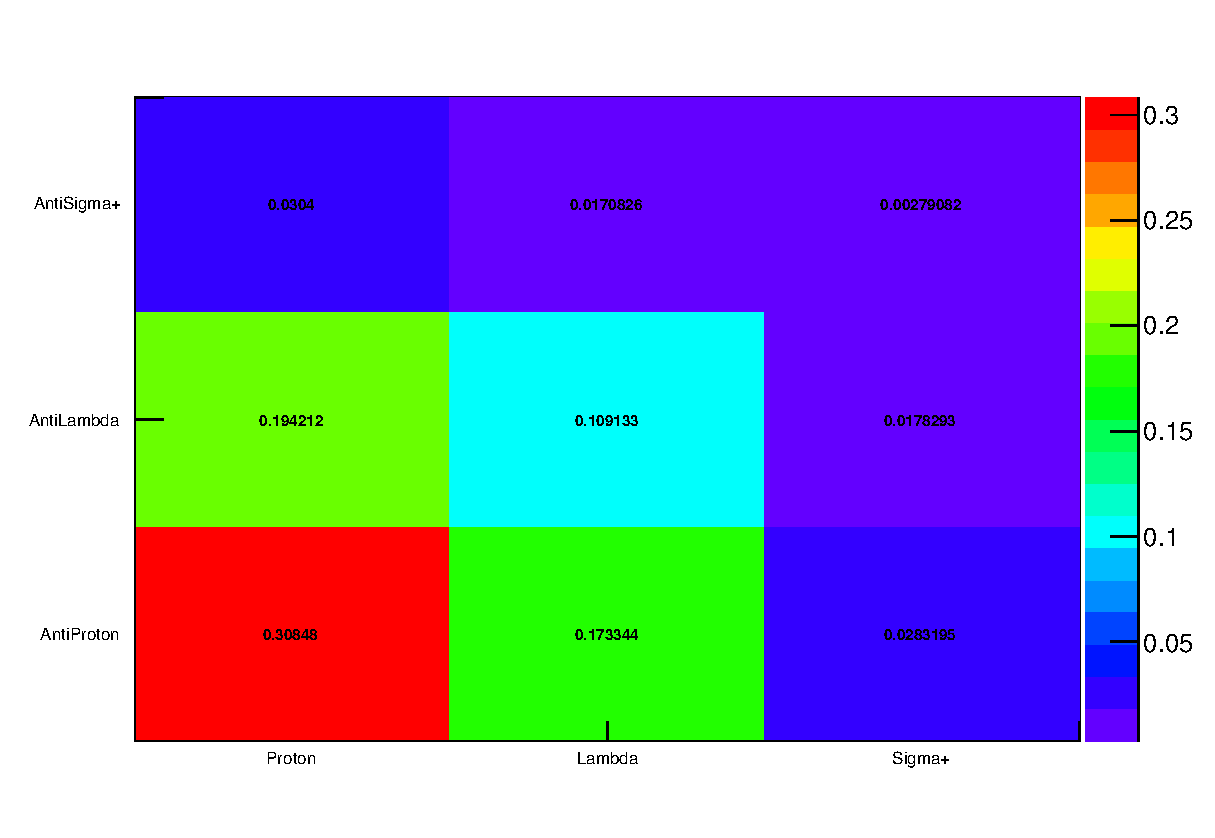
\includegraphics[width=0.99\textwidth]{pics/papFractionTherm}
   \caption{Therminator2 \pap~fraction}
   \label{fig:papFractionTherm}
 \end{figure}

  \begin{figure}[h!]
   \centering
   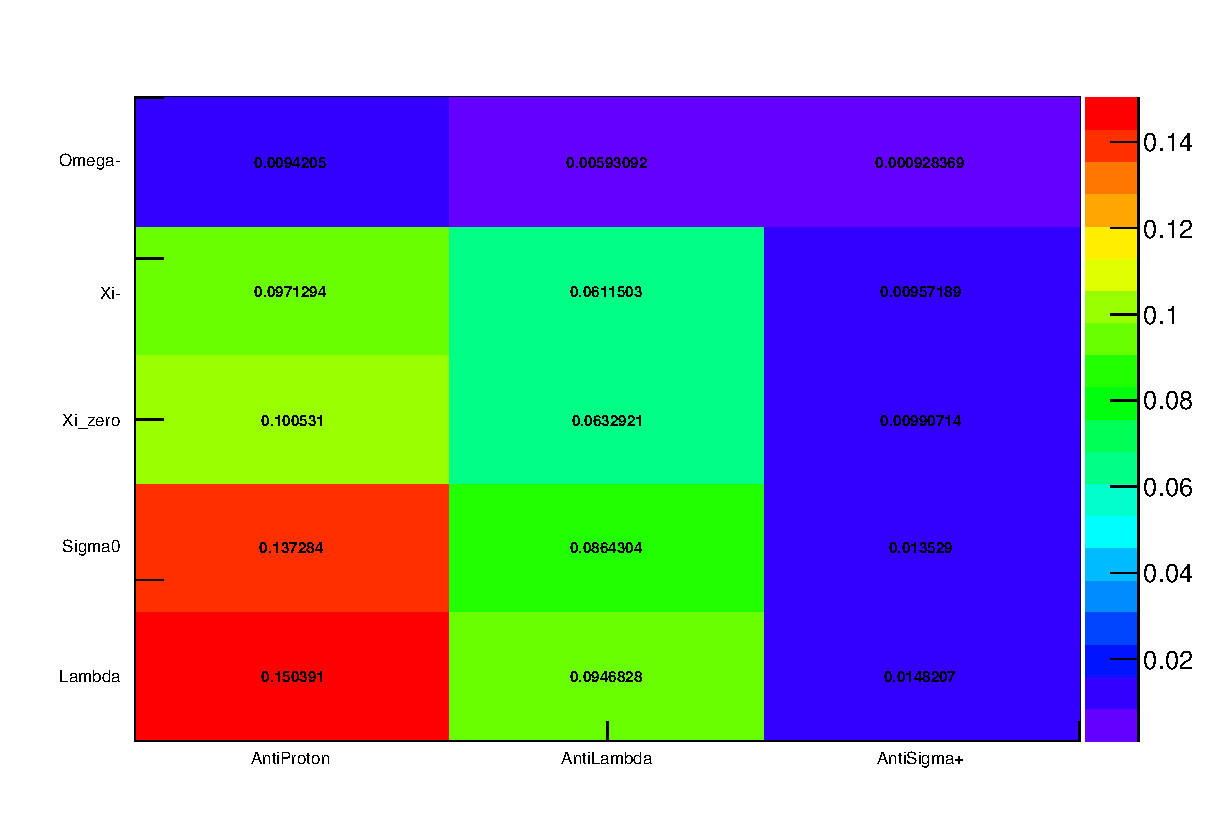
\includegraphics[width=0.99\textwidth]{pics/aplFractionTherm}
   \caption{Therminator2 \apl~fraction}
   \label{fig:aplFractionTherm}
 \end{figure}

 \begin{figure}[h!]
   \centering
   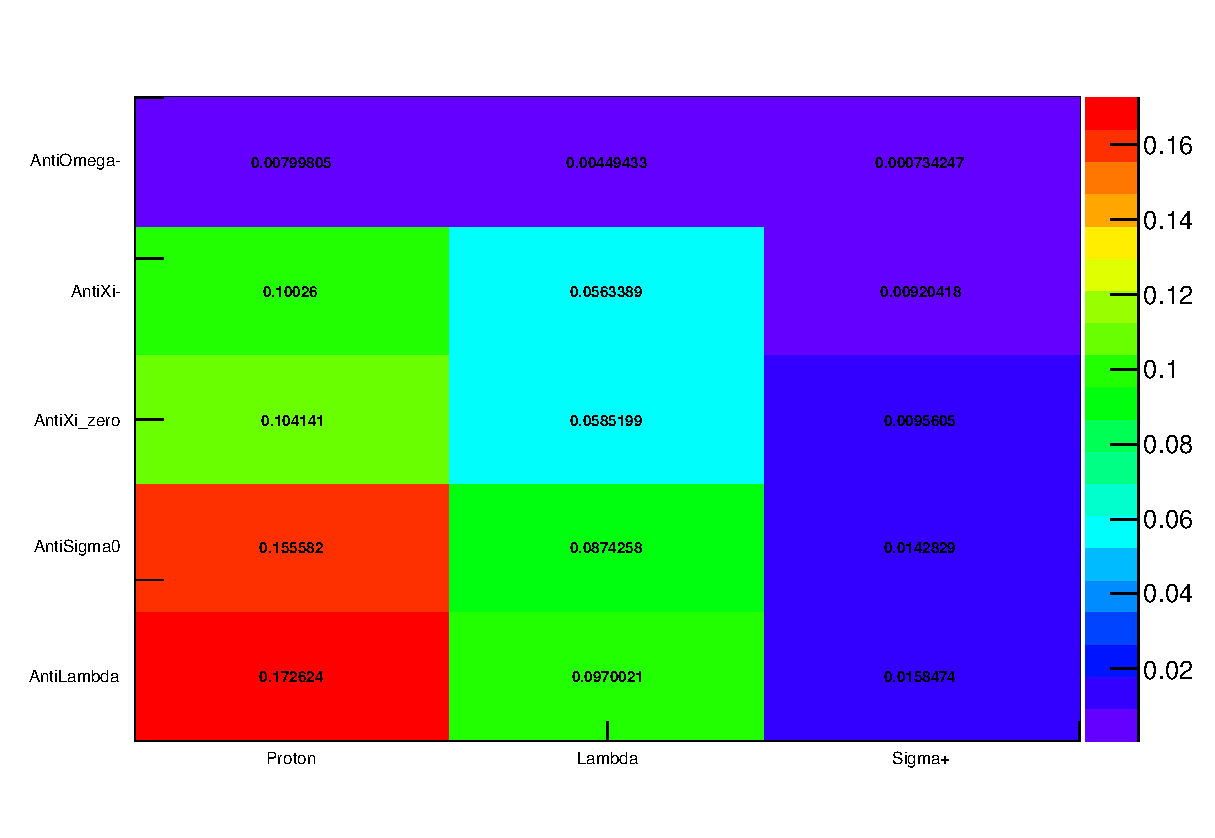
\includegraphics[width=0.99\textwidth]{pics/palFractionTherm}
   \caption{Therminator2 \pal~fraction}
   \label{fig:palFractionTherm}
 \end{figure}

%% \begin{frame}% [<+->]
%%   {\pap~fractions (Therminator)}
%%   \begin{center}
%%     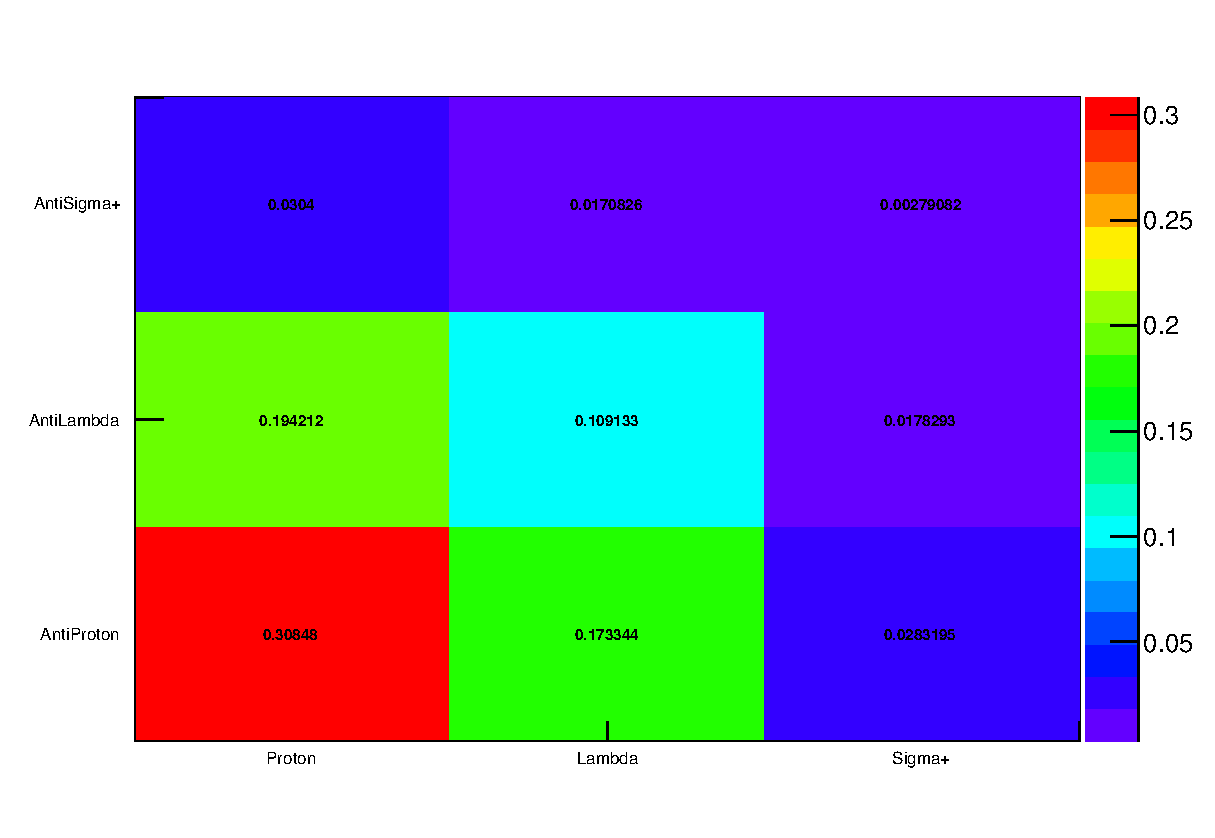
\includegraphics[width=0.9\textwidth]{pics/papFractionTherm}
%%   \end{center}
%% \end{frame}

%% \begin{frame}% [<+->]
%%   {\apl~fractions (Therminator)}
%%   \begin{center}
%%     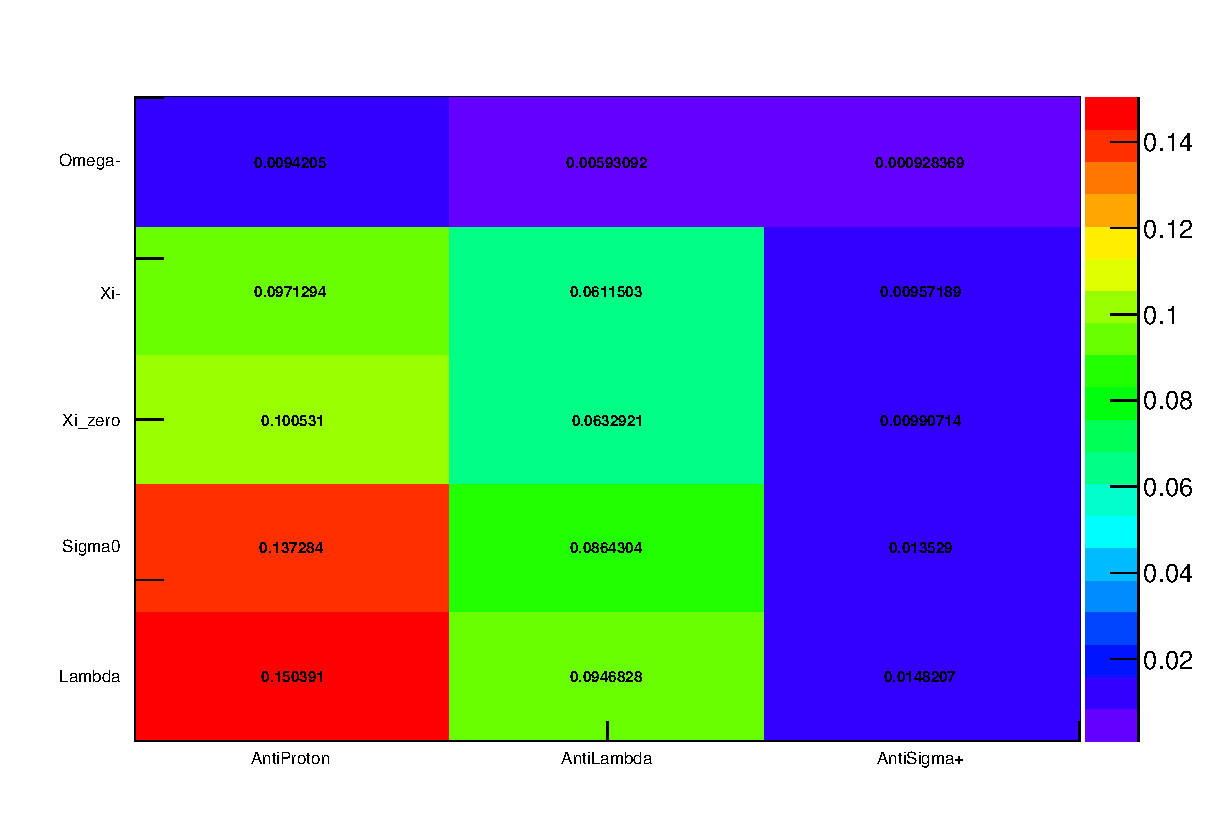
\includegraphics[width=0.9\textwidth]{pics/aplFractionTherm}
%%   \end{center}
%% \end{frame}

%% \begin{frame}% [<+->]
%%   {\pal~fractions (Therminator)}
%%   \begin{center}
%%     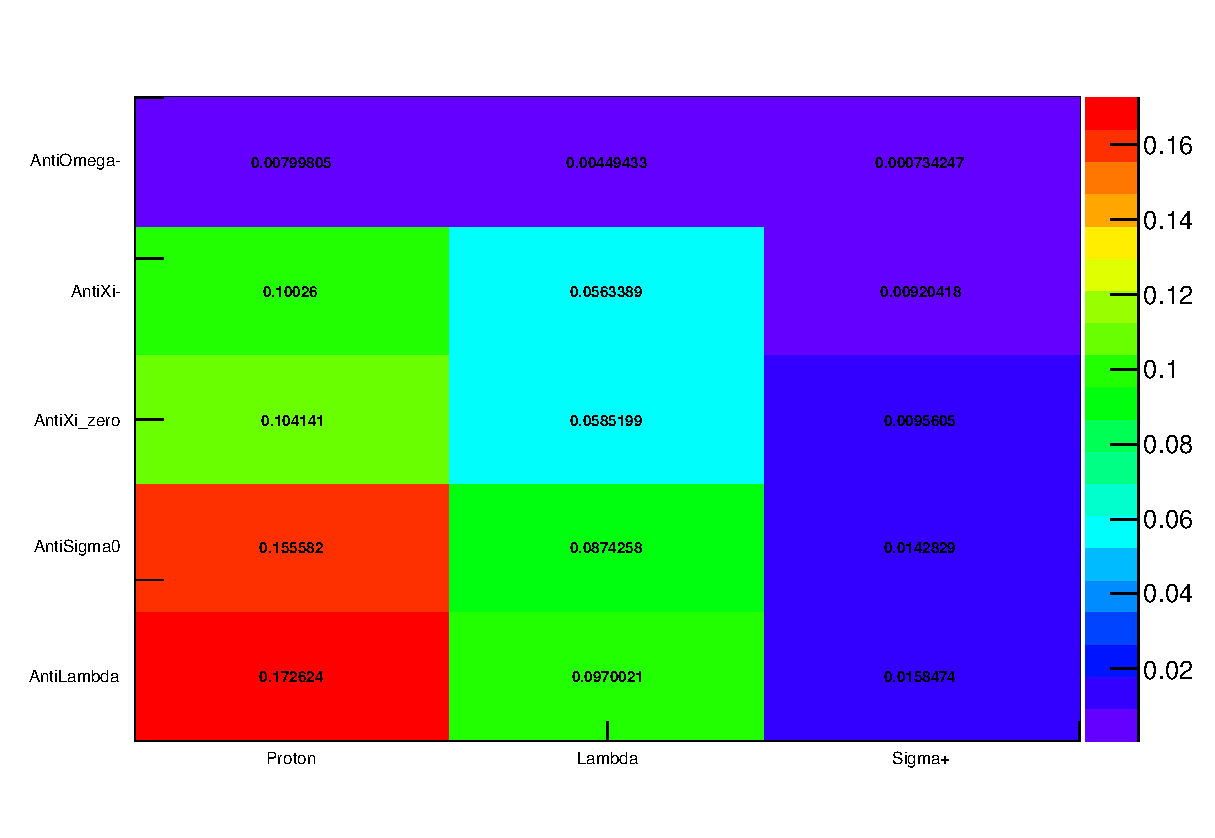
\includegraphics[width=0.9\textwidth]{pics/palFractionTherm}
%%   \end{center}
%% \end{frame}

DCA cut ?!

\section{Results}

\subsection{Correlation functions}

\subsubsection{Comparison of magnetic field orientations}

\begin{figure}[]
   \centering
   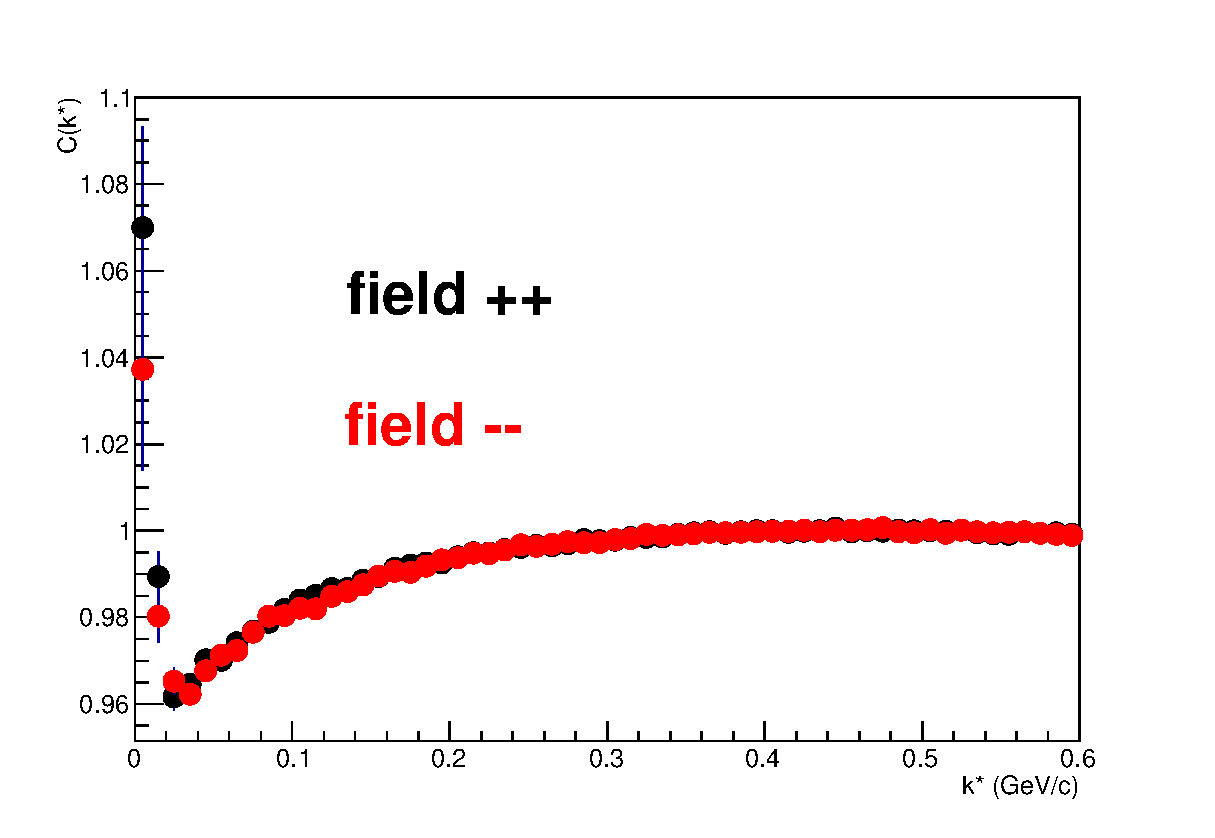
\includegraphics[width=0.99\textwidth]{pics/compPAP}
   \caption{ \pap~correlation function, centrality 0-10$\%$, magnetic field comparison}
   \label{fig:papCorrFun}
 \end{figure}

\begin{figure}[]
   \centering
   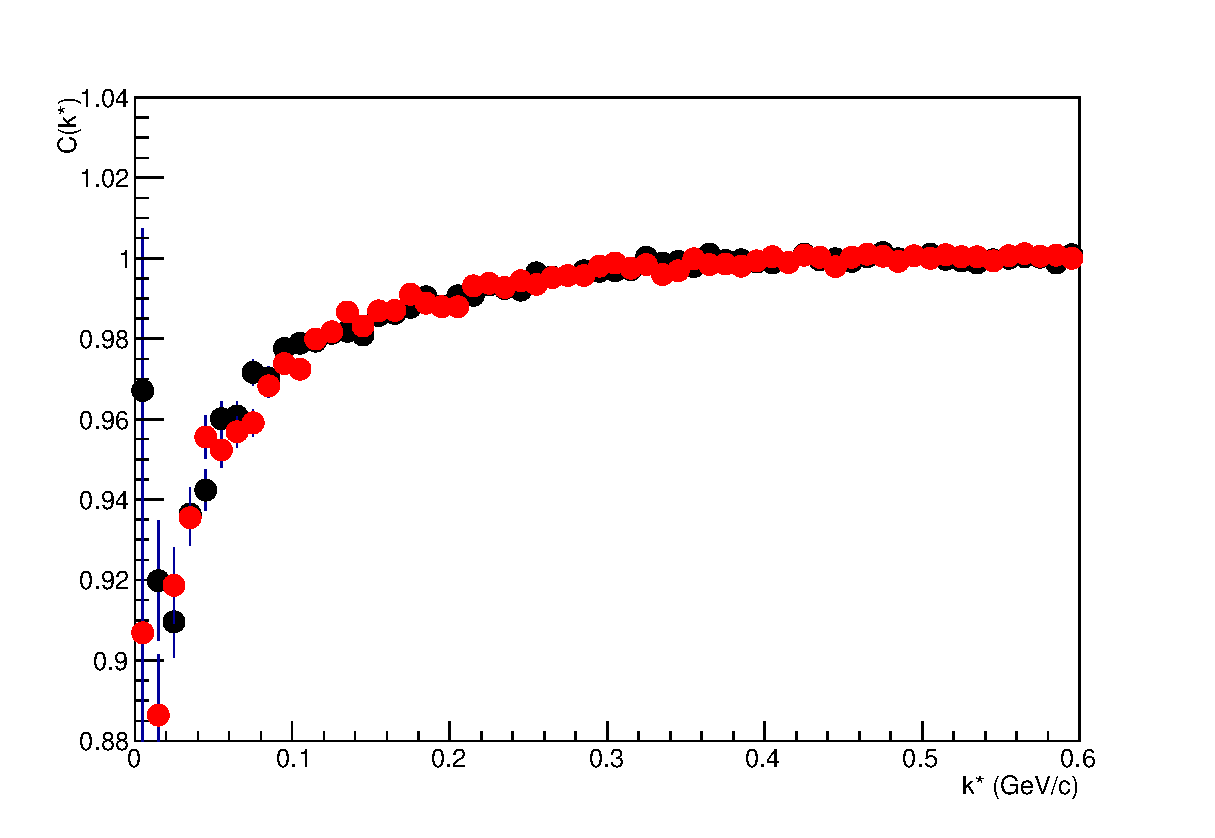
\includegraphics[width=0.99\textwidth]{pics/compPAL}
   \caption{ \pal~correlation function, centrality 0-10$\%$, magnetic field comparison}
   \label{fig:palCorrFun}
 \end{figure}

\begin{figure}[]
   \centering
   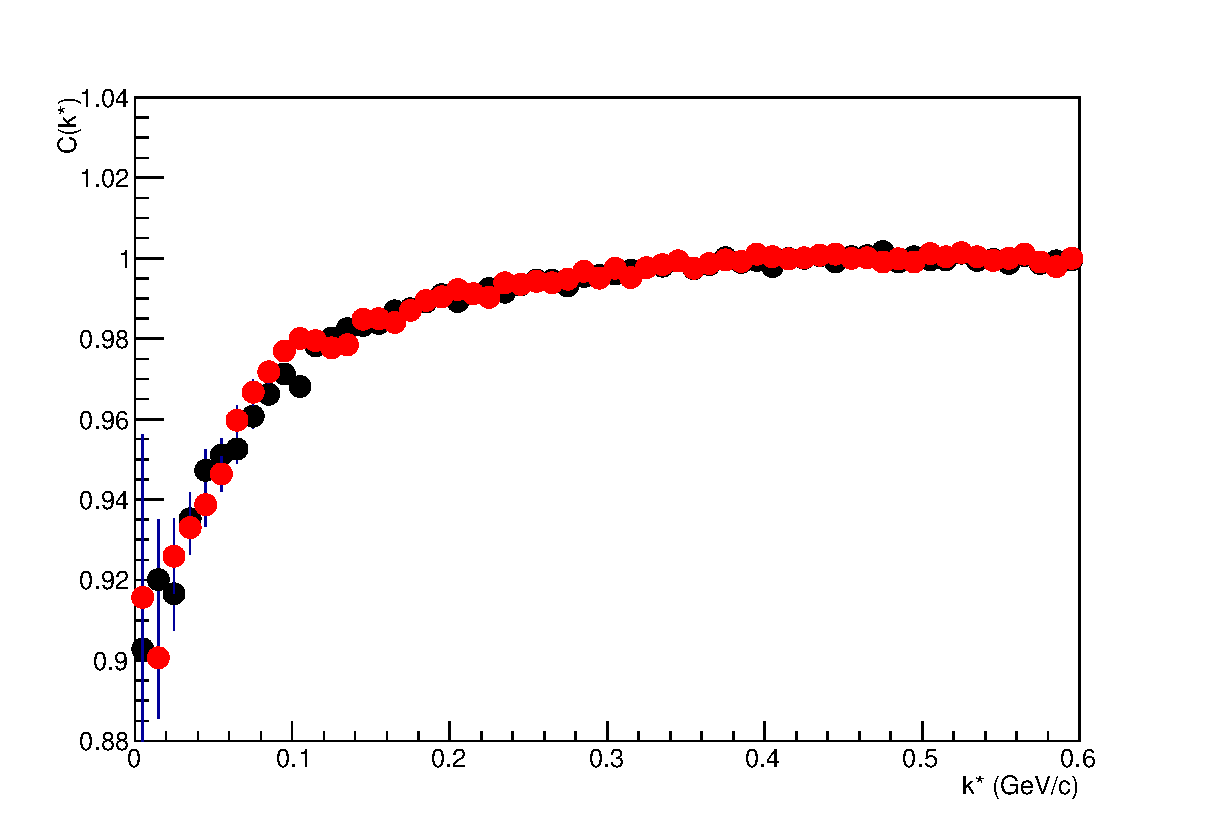
\includegraphics[width=0.99\textwidth]{pics/compAPL}
   \caption{ \apl~correlation function, centrality 0-10$\%$, magnetic field comparison}
   \label{fig:aplCorrFun}
 \end{figure}

\subsubsection{Non-femtoscopic background}

\begin{figure}[]
   \centering
   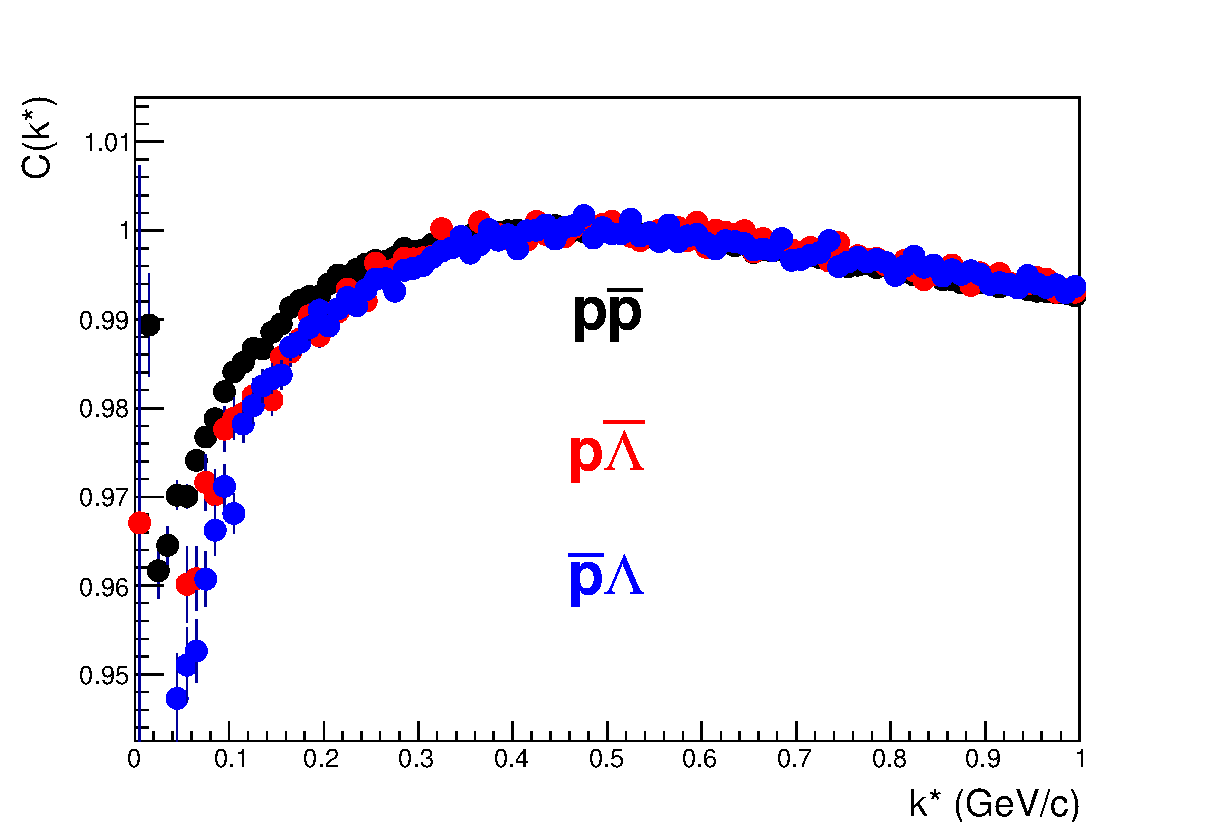
\includegraphics[width=0.99\textwidth]{pics/compBack010}
   \caption{ Non-femtoscopic background in~\pap,~\pal,~\apl,~centrality 0-10$\%$}
   \label{fig:backCorrFun010}
 \end{figure}

\begin{figure}[]
   \centering
   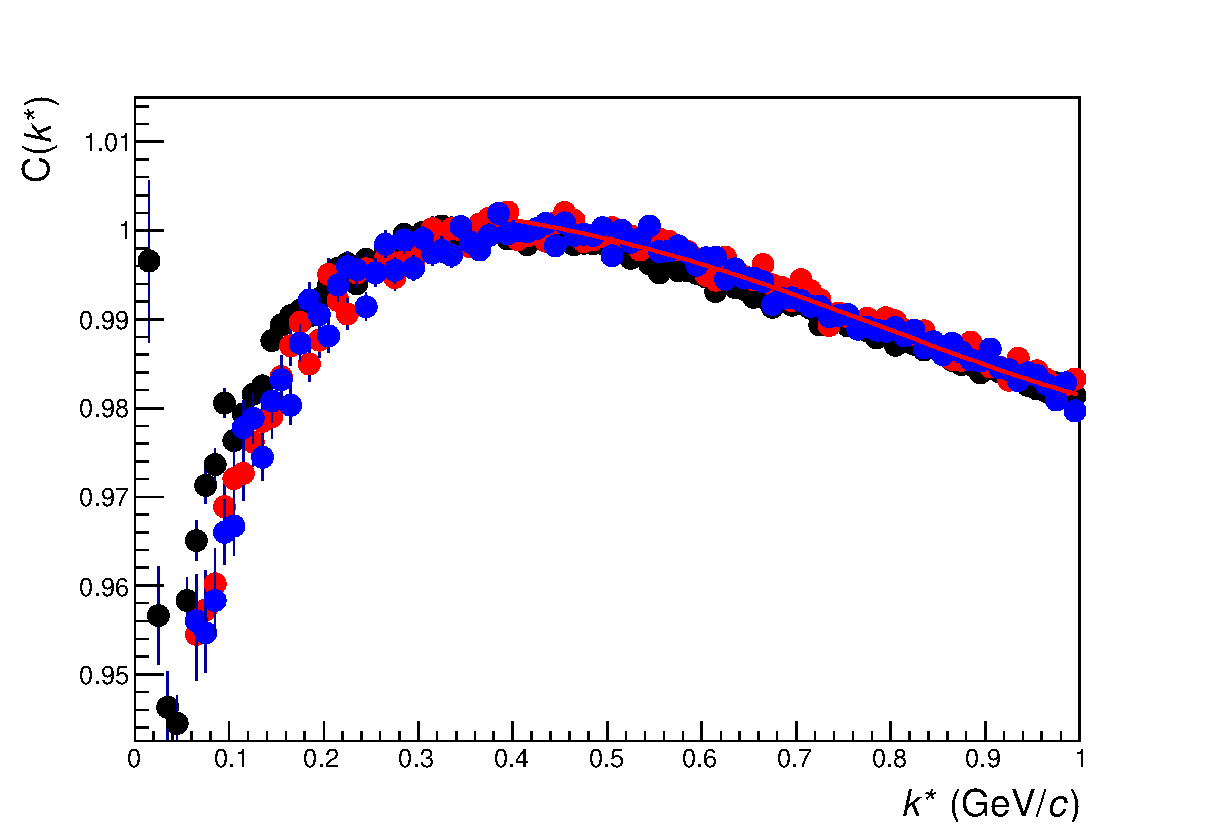
\includegraphics[width=0.99\textwidth]{pics/compBack1030}
   \caption{ Non-femtoscopic background in \pap,~\pal,~\apl, centrality 10-30$\%$}
   \label{fig:backCorrFun1030}
 \end{figure}

\begin{figure}[]
   \centering
   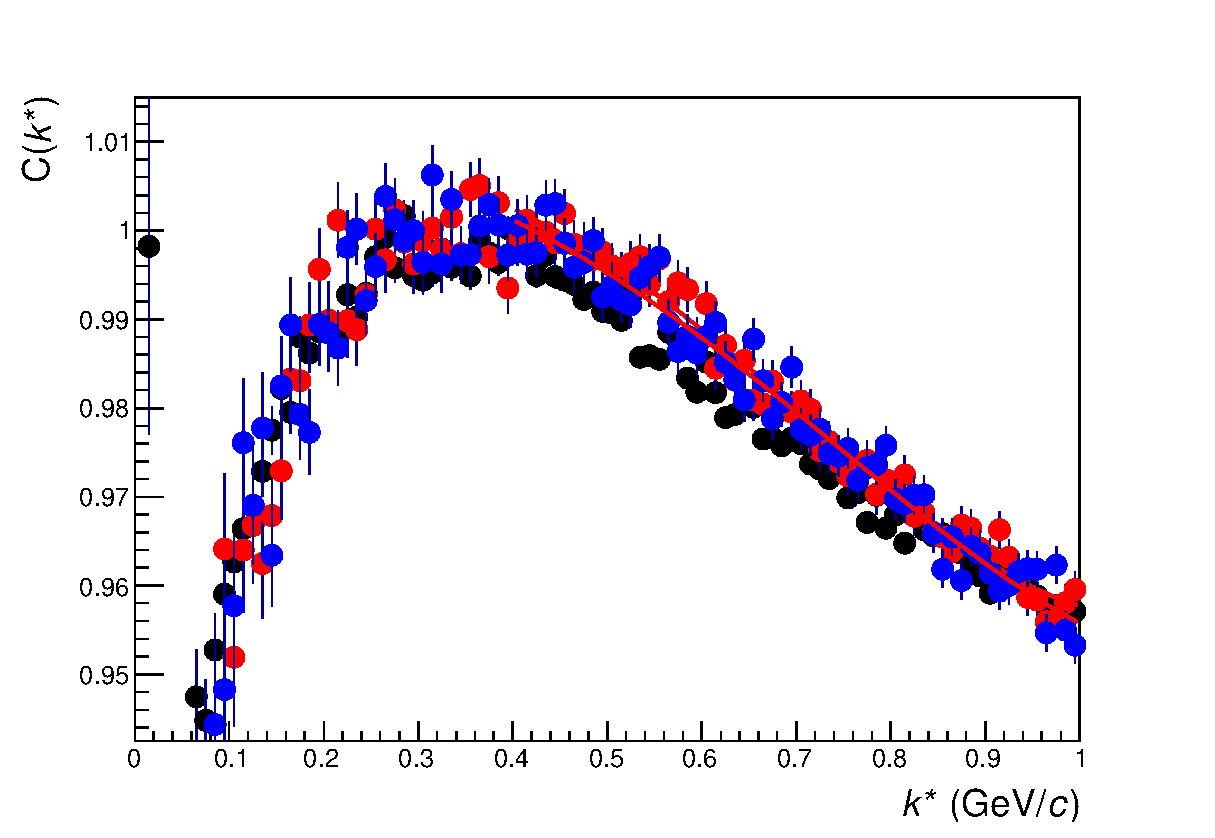
\includegraphics[width=0.99\textwidth]{pics/compBack3050}
   \caption{ Non-femtoscopic background in \pap,~\pal,~\apl, centrality 30-50$\%$}
   \label{fig:backCorrFun3050}
 \end{figure}

\subsubsection{Event plane selection method}

\subsubsection{Correlation function from Monte Carlo}

\begin{figure}[]
   \centering
   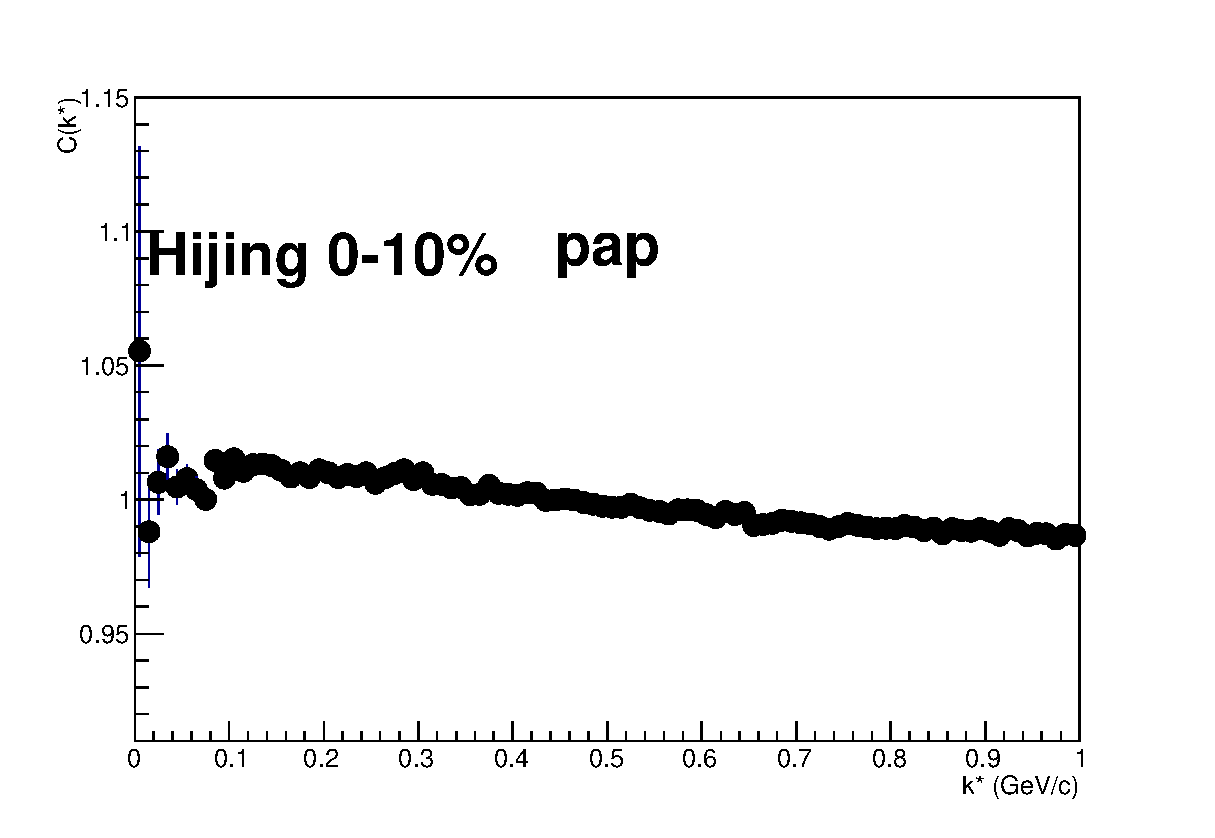
\includegraphics[width=0.99\textwidth]{pics/hijingpap}
   \caption{ \pap~correlation function, centrality 0-10$\%$, hijing}
   \label{fig:papCorrFunHijng}
 \end{figure}

\begin{figure}[]
   \centering
   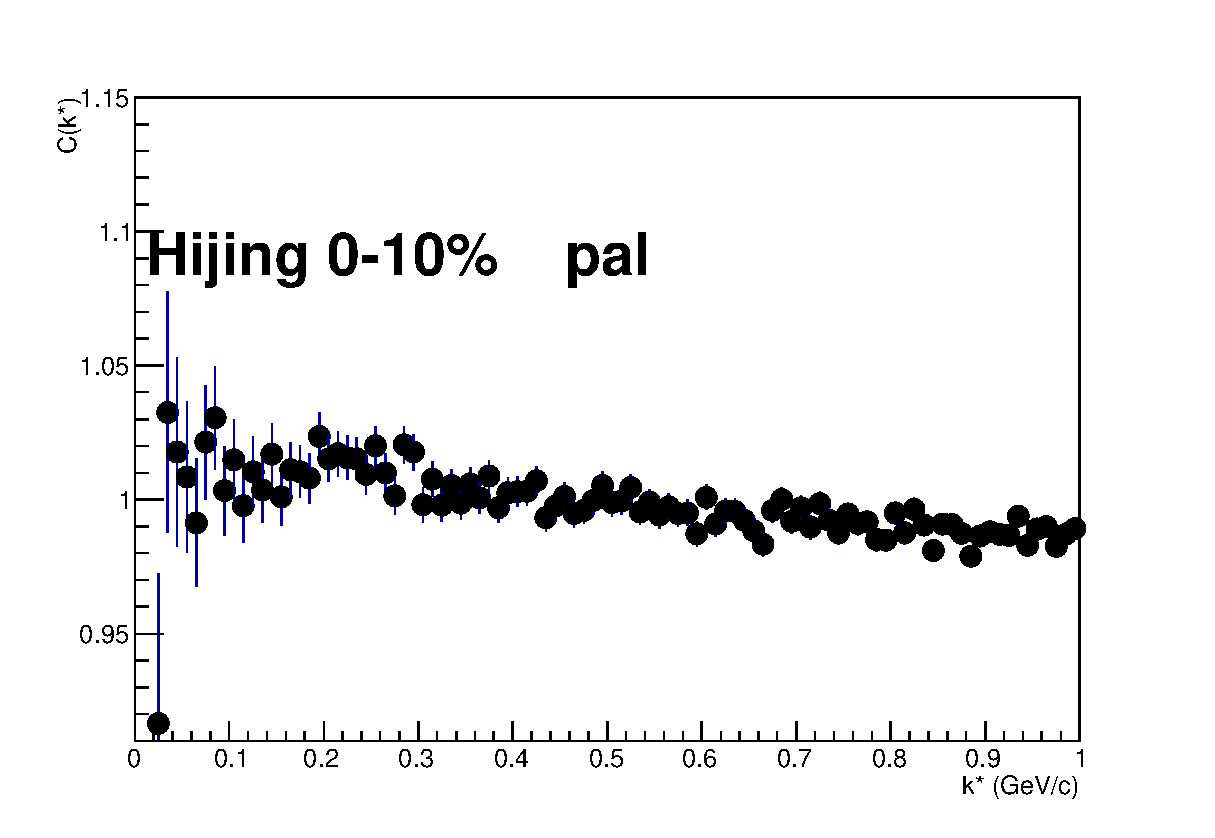
\includegraphics[width=0.99\textwidth]{pics/hijingpal}
   \caption{ \pal~correlation function, centrality 0-10$\%$, hijing}
   \label{fig:palCorrFunHijing}
 \end{figure}

\begin{figure}[]
   \centering
   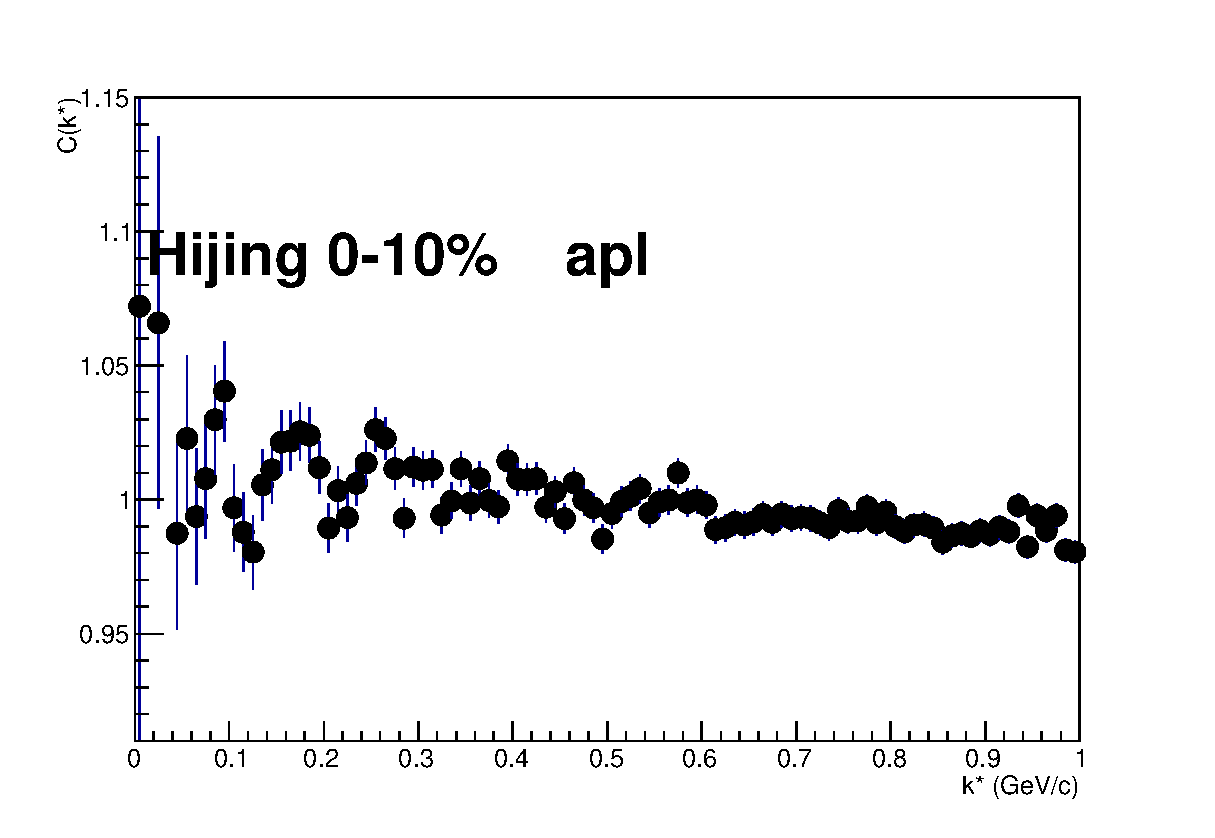
\includegraphics[width=0.99\textwidth]{pics/hijingapl}
   \caption{ \apl~correlation function, centrality 0-10$\%$, hijing}
   \label{fig:aplCorrFunHijing}
 \end{figure}

\subsection{Fitting procedure}

\subsubsection{Residual correlations}

\subsubsection{\pap~theoretical function}

\paragraph{Gaussian source}

\begin{figure}[]
   \centering
   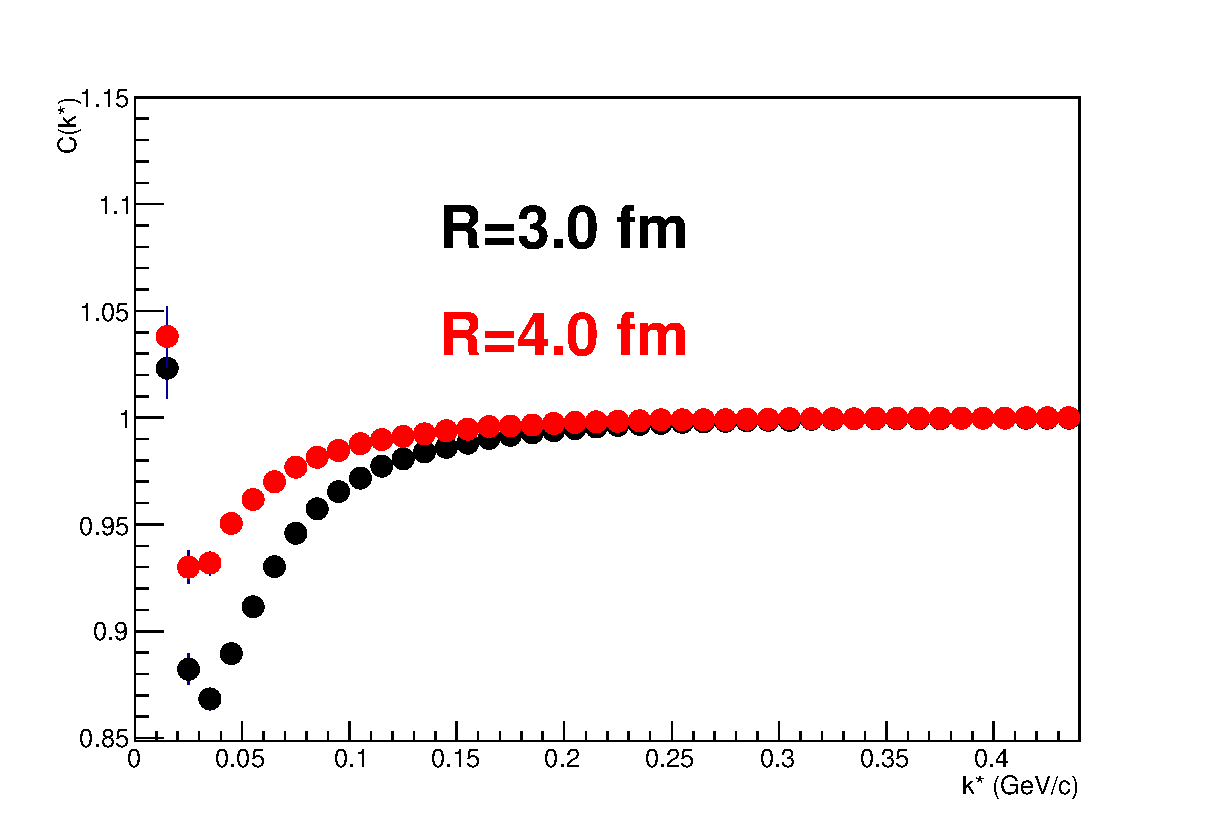
\includegraphics[width=0.99\textwidth]{pics/pap.eps}
   \caption{\pap~correlation function generated using Lednicky's weights and assuming Gaussian source.}
   \label{fig:cfpapgaus}
 \end{figure}

\paragraph{Therminator source}

\begin{figure}[]
   \centering
   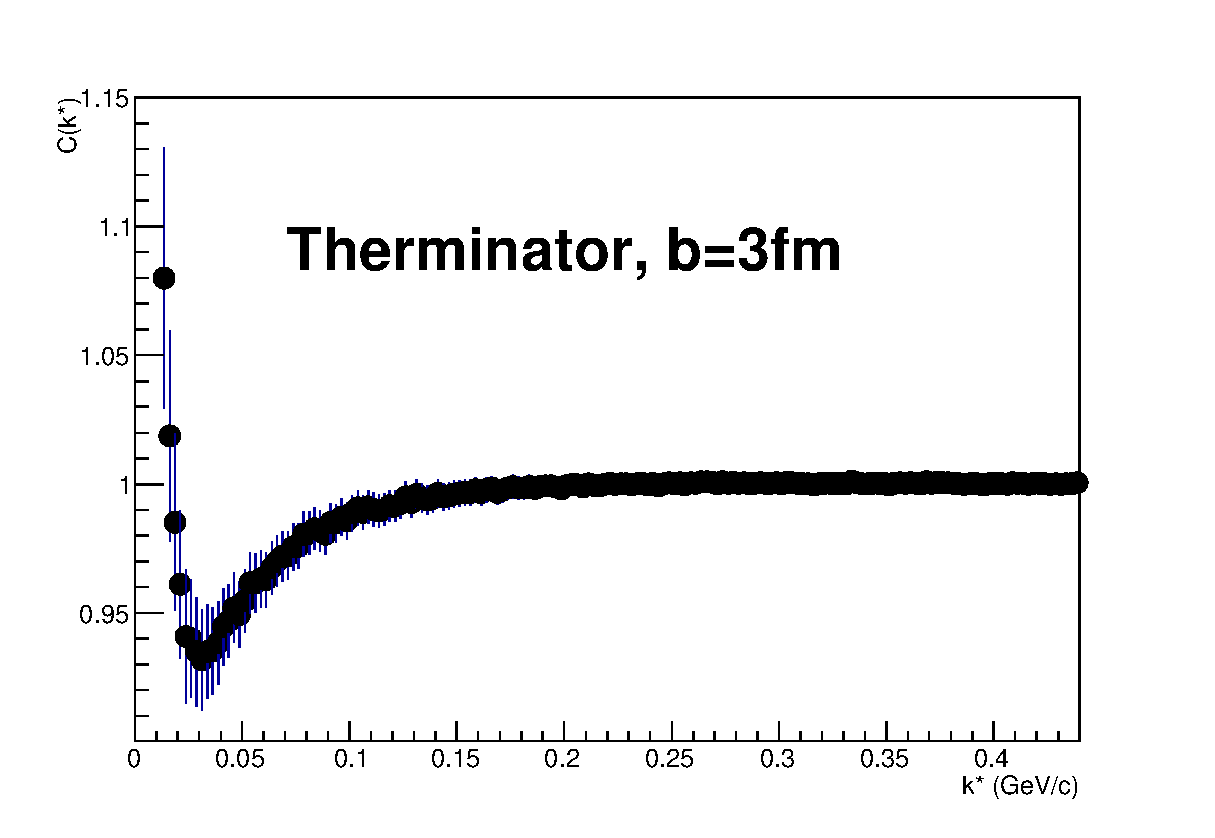
\includegraphics[width=0.99\textwidth]{pics/paptherm.eps}
   \caption{\pap~correlation function generated using source from Therminator simulation and Lednicky's weights.}
   \label{fig:cfpaptherm}
 \end{figure}

\subsubsection{\pal~and \apl~theoretical function}

\subsubsection{Fitting results}

\begin{figure}[]
   \centering
   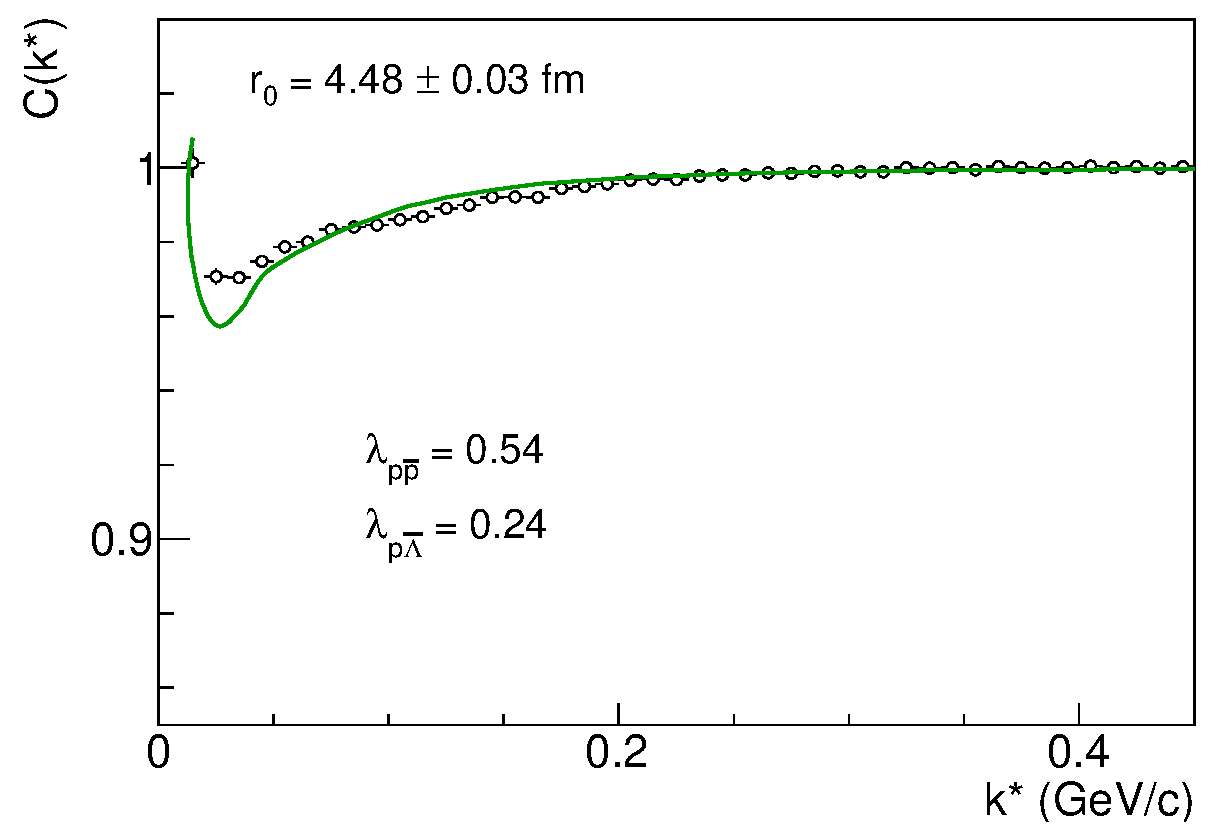
\includegraphics[width=0.99\textwidth]{pics/divp4NumOutPckstarPAPtpcM0Psi3_fitpap0.eps}
   \caption{Fit to \pap~correlation function divided by pol4, centrality 0-10$\%$}
   \label{fig:fitpap0}
 \end{figure}

\begin{figure}[]
   \centering
   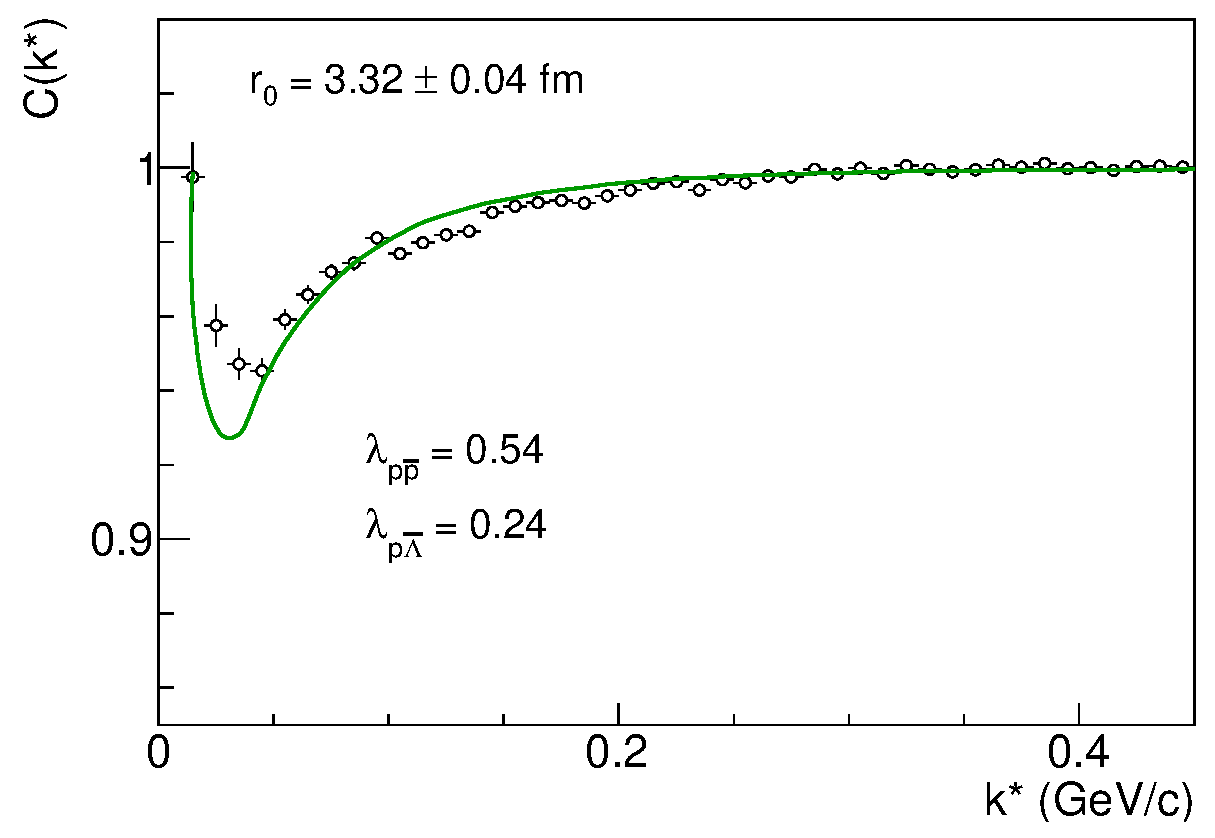
\includegraphics[width=0.99\textwidth]{pics/divp4NumOutPckstarPAPtpcM2Psi3_fitpap1.eps}
   \caption{Fit to \pap~correlation function divided by pol4, centrality 10-30$\%$}
   \label{fig:fitpap1}
 \end{figure}

\begin{figure}[]
   \centering
   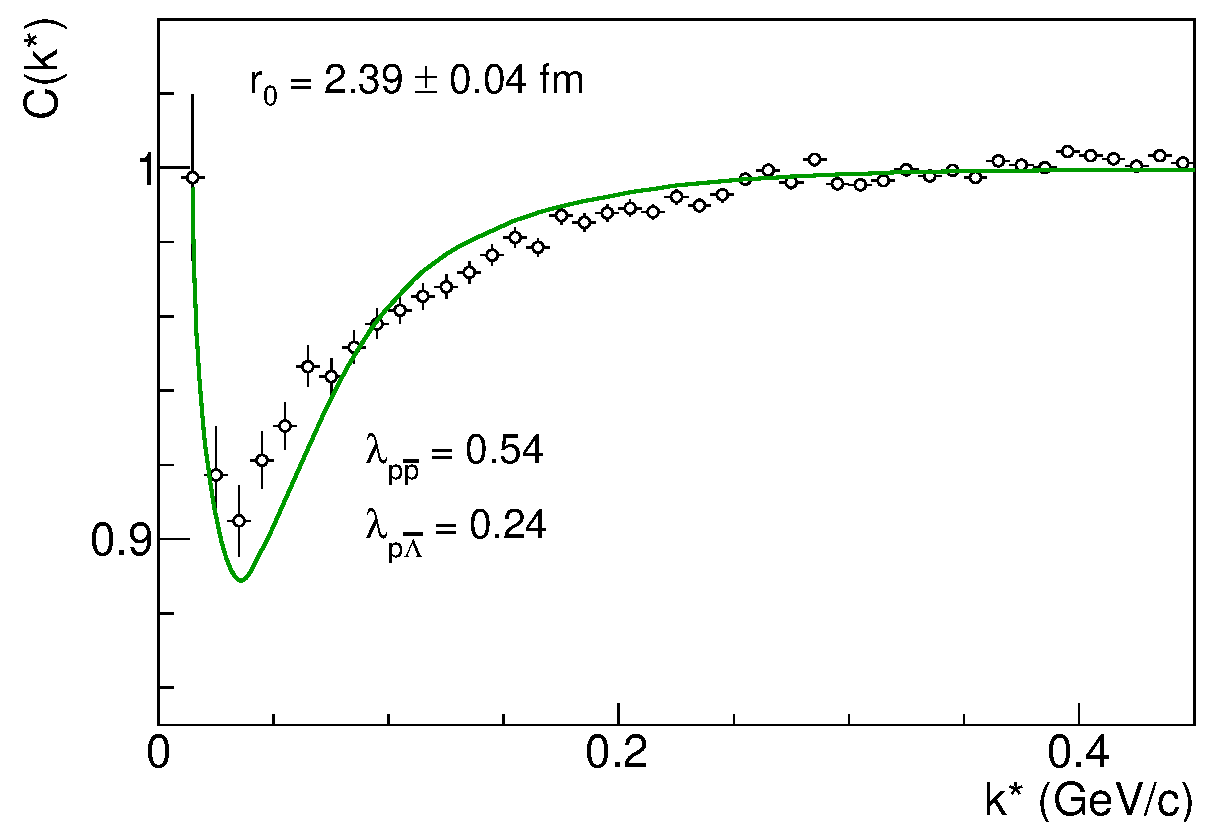
\includegraphics[width=0.99\textwidth]{pics/divp4NumOutPckstarPAPtpcM4Psi3_fitpap2.eps}
   \caption{Fit to \pap~correlation function divided by pol4, centrality 30-50$\%$}
   \label{fig:fitpap2}
 \end{figure}

\paragraph{AQM}

\paragraph{Simultaneous}

\paragraph{Global}

\paragraph{R fixed}

\paragraph{f0 fixed}

\subsection{Systematic uncertainties}

\subsubsection{ non-femtoscopic background}
\subsubsection{ fractions (Hijing vs. Therminator)}
\subsubsection{ number of secondaries from material}
\subsubsection{ momentum resolution correction}
\subsubsection{ ALICE magnetic fields ++ vs. - - }
\subsubsection{ PID}
\subsubsection{ different scenarios for interaction parameters}
\subsubsection{ DCA templates}
\subsubsection{ \pal~vs.~\apl}
\subsubsection{ fitting procedure    }

\subsubsection{Momentum resolution}
Correction for momentum resolution is taken into account in the fitting procedure. Fit function is smeared with a gaussian function with the width corresponding the momentum resolution for the pairs of interest. Following formula is used:
\begin{equation}
  C_c(q_c) = \int_{-3\sigma}^{+3\sigma}C_{th}(q_c-q) Gaus(q_t, \sigma)(q) |q_c-q|^2 d q,
\end{equation}
where $C_c$ is the corrected function, $C_{th}$ is the ideal function, $\sigma$ is the momentum resolution.

\bibliographystyle{utphys}   % Put here the style file name for the paper, i.e.apsrev4-1, utphys
\bibliography{ALICE_analysis_note}

\end{document}
